\documentclass{jsarticle}
\usepackage[dvipdfmx]{graphicx}
\usepackage{bm}
\usepackage{amsmath}
\usepackage{amssymb}
\usepackage{amsfonts}
\usepackage{comment}
\usepackage{listings}
\usepackage{cases}
\lstset{
    basicstyle={\ttfamily},
    identifierstyle={\small},
    commentstyle={\smallitshape},
    keywordstyle={\small\bfseries},
    ndkeywordstyle={\small},
    stringstyle={\small\ttfamily},
    frame={tb},
    breaklines=true,
    columns=[l]{fullflexible},
    numbers=left,
    xrightmargin=0zw,
    xleftmargin=3zw,
    numberstyle={\scriptsize},
    stepnumber=1,
    numbersep=1zw,
    lineskip=-0.5ex,
    keepspaces=true,
    language=c
}
\renewcommand{\lstlistingname}{リスト}
\makeatletter
\newcommand{\figcaption}[1]{\def\@captype{figure}\caption{#1}}
\newcommand{\tblcaption}[1]{\def\@captype{table}\caption{#1}}
\makeatother

\title{数値解析レポートNo.3}
\author{32番 平田 蓮}
\date{}

\begin{document}
\maketitle
    \section{指数近似}
        指数近似$y = a_0e^{a_1x}$について、両辺対数を取ると、$\ln y = \ln a_0 + a_1x$となる。
        この式は多項式近似と同じ形であるので、$a_0, a_1$を求めることができる。
        これを元に指数近似を行う関数\verb|exp_approximation()|をリスト\ref{src:exp}に示す。

        \begin{lstlisting}[caption=exp\_approximation, label=src:exp]
#define A_NUM 2    / / coefficient number
#define DATA_NUM 4 / / sample number

double *exp_approxmation(
    double *x, / / sample x coordinates
    double *y  / / sample y coordinates
) {
    double
        *a = allocVector(A_NUM),
        *b = allocVector(A_NUM),
        **A = allocMatrix(A_NUM, A_NUM);

    for (i = 0; i < A_NUM; i++) {
        for (j = 0; j < DATA_NUM; j++) {
            b[i] += log(y[j]) * pow(x[j], i);
        }
    }

    for (i = 0; i < A_NUM; i++) {
        for (j = i; j < A_NUM; j++) {
            for (k = 0; k < DATA_NUM; k++) {
                A[i][j] += pow(x[k], i + j);
            }
            A[j][i] = A[i][j];
        }
    }

    gauss(A, b, A_NUM, A_NUM); / / gaussian elimination
    backward_substitution(A, b, a, A_NUM); / / backward substitution
    a[0] = exp(a[0]);

    return a;
}\end{lstlisting}

        与えられたデータを近似すると、$a_0 \approx 2, a_1 \approx 1$が得られる。
        与えられたデータと$y = 2e^x$をプロットしたものを図\ref{fig:exp}に示す。

        \begin{figure}[h]
            \centering
            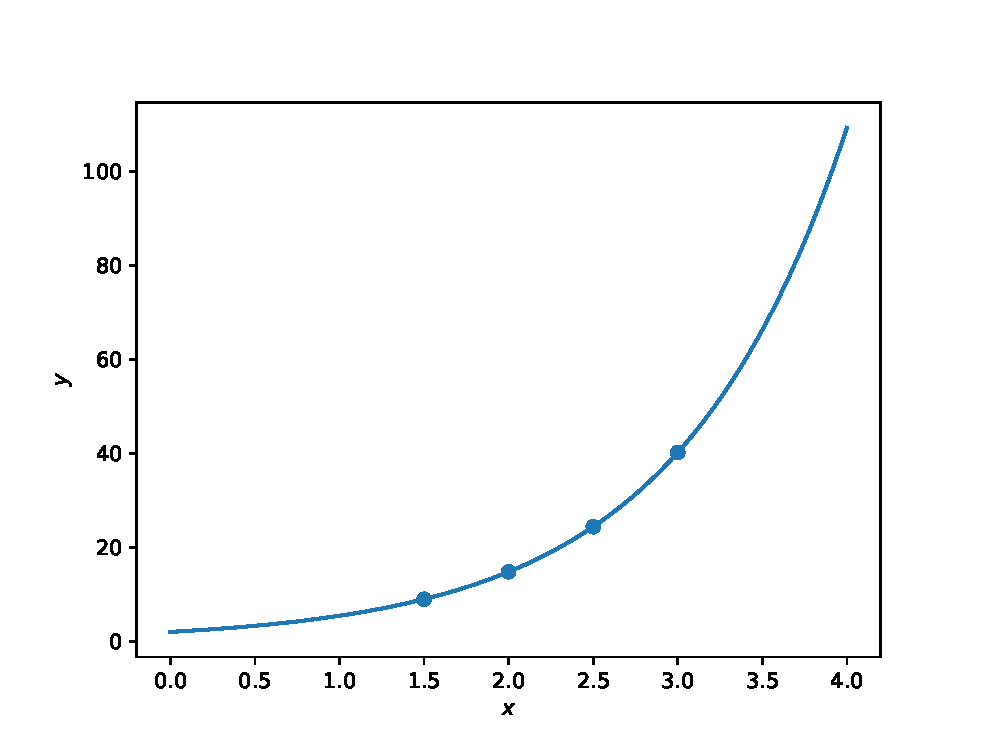
\includegraphics[width=0.8\hsize]{img/exp.eps}
            \caption{指数近似}
            \label{fig:exp}
        \end{figure}

    \section{サービス問題}
        \subsection{良いところ$\cdot$参考になったところ}
            他人のコードを読むにあたって、
            特にコメントの書き方は興味深かった。
            自分は普段あまりコメントを書かないので、
            他人に伝わりやすいコメントという観点でとても参考になったところもあった。

            また、他人のコードを読むことで同じアルゴリズムでも少し違った
            実装の仕方を発見できたり、今後のプログラミングに活かせそうな学びを得ることができた。

        \subsection{感想}
            特に、プログラムの汎用性という部分であまり上手にプログラムを書けない人が
            多い印象であった。自作関数、構造体など、
            汎用性を高めるためのパーツはこれまでの授業で扱ったが、
            実際にそれらを利用して
            汎用性のないプログラムにどのように汎用性を持たせることができるかといった
            内容の講義があればよりクラスのプログラミング力が向上するのではないかと思った。
    
    \section{数値積分の比較}
        台形公式、シンプソン公式、ロンバーグ積分の三つの手法で定積分を行う関数をリスト\ref{src:int}に示す。

        \begin{lstlisting}[caption=integral.c, label=src:int]
double trapezoid(
    double (*f)(double), / / function
    double a, / / start
    double b, / / end
    int n / / partition number
) {
    if (a > b) return -trapezoid(f, b, a, n);
    double sum = 0, dx = (b - a) / n, x;
    for (x = a; x <= b; x += dx) {
        sum += f(x);
    }
    sum -= (f(a) + f(b)) / 2.0;
    return sum * dx;
}

double simpson(
    double (*f)(double), / / function
    double a, / / start
    double b, / / end
    int n / / partition number
) {
    if (a > b) return -simpson(f, b, a, n);
    double sum = 0, dx = (b - a) / n, x;
    sum = f(a) + f(b);
    for (x = a + dx; x <= b; x += dx) {
        sum += 4.0 * f(x - dx / 2.0) + 2.0 * f(x);
    }
    sum -= 2.0 * f(b);
    
    return sum * dx / 6.0;
}

double romberg(
    double (*f)(double), / / function
    double a, / / start
    double b, / / end
    int n / / partition number
    double **T / / 2d array for calculation
) {
    if (a > b) return -romberg(f, a, b, n, T);
    int k, m;
    double h, x;

    T[0][0] = (b - a) * (f(a) + f(b)) / 2.0;

    for (k = 1; k < n; k++) {
        h = (b - a) / pow(2, k);

        T[k][0] = T[k - 1][0] / 2.0;
        for (x = a + h; x <= b - h; x += 2.0 * h) {
            T[k][0] += h * f(x);
        }

        for (m = 1; m <= k; m++) {
            T[k][m] = T[k][m - 1] + (T[k][m - 1] - T[k - 1][m - 1]) / (pow(4.0, m) - 1.0);
        }
    }

    return T[n - 1][n - 1];
}\end{lstlisting}

    \subsection{分割数の増加による誤差の推移}
        このプログラムを使って$y = \sin x \ (0 \le x \le \displaystyle\frac{\pi}{2})$、
        $y = x \ln x \ (0 \le x \le e)$の定積分を求める。

        まず理論値を求める。
        $y = \sin x$について、$\displaystyle\int_0^{\frac{\pi}{2}} \sin x dx = 1$
        となる。
        $y = x\ln x$については広義積分を行い、
        $\displaystyle\int_0^e x \ln x dx = \left[\frac{x^2\ln x}{2} - \frac{x^2}{4}\right]_0^e = \frac{e^2}{4} \approx 1.847264$となる。

        図\ref{fig:sinx}、\ref{fig:xlnx}に各分割数について定積分の計算結果と理論値との差をプロットしたものを示す。

        \begin{figure}[h]
            \begin{minipage}{0.5\hsize}
                \centering
                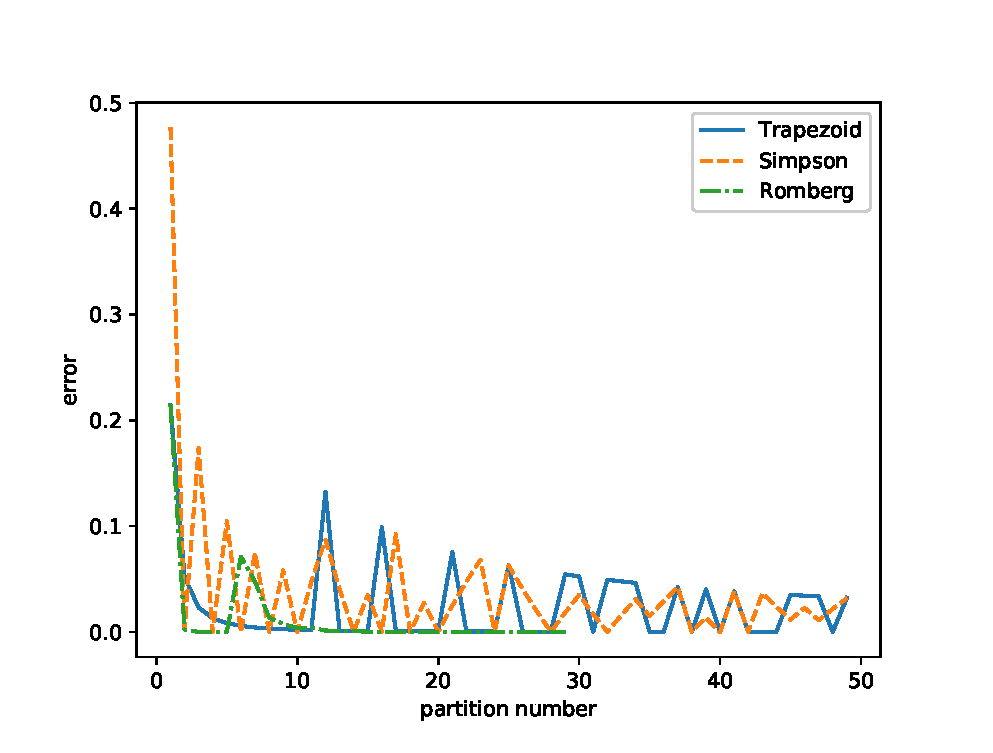
\includegraphics[width=1\hsize]{img/sinx.eps}
                \caption{$y = \sin x$の定積分の誤差の推移}
                \label{fig:sinx}
            \end{minipage}
            \begin{minipage}{0.5\hsize}
                \centering
                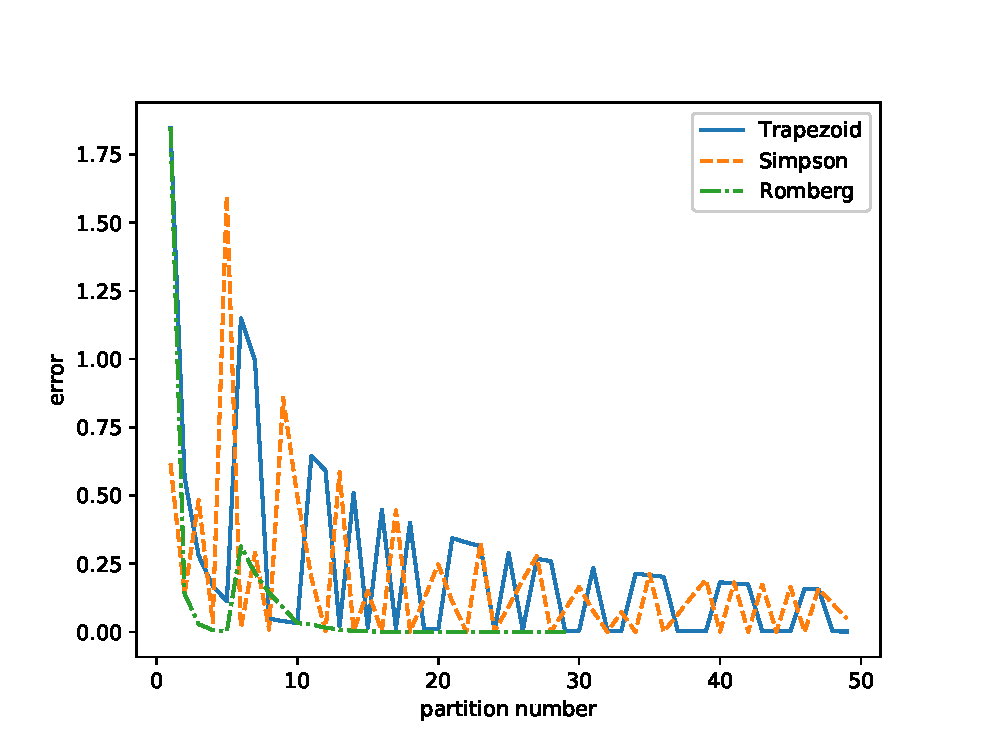
\includegraphics[width=1\hsize]{img/xlnx.eps}
                \caption{$y = x\ln x$の定積分の誤差の推移}
                \label{fig:xlnx}
            \end{minipage}
        \end{figure}

        図より、ロンバーグ積分、シンプソン公式、台形公式の順に収束が早いことがわかる。
        また、分割数が大きくなっても台形公式とシンプソン公式は誤差が出ることがあるが、ロンバーグ積分は完全に収束する。
        関数と分割数の相性によっては台形公式やシンプソン公式の方が小さい分割数で誤差がロンバーグ積分より少なくなる場合もあることがわかる。

    \subsection{各手法の計算量}
        リスト\ref{src:int}を見ればわかるように、台形公式とシンプソン公式の計算量は
        分割数$N$に対して$O(N)$である。
        対してロンバーグ積分は$\displaystyle O\left(\sum_{k = 0}^{N - 1} 2^{k}\right) = O\left(2^N\right)$であるので、
        現実的に計算可能なロンバーグ積分は$N = 30$前後である。
        
        しかし、誤差の小ささをみると、台形公式やシンプソン公式よりロンバーグ積分を使う方が良いと考えられる。
        台形公式とシンプソン公式は関数と相性の良い分割数についてはほぼ誤差がない値を導けるが、
        そうでない分割数についてはある程度の誤差を出してしまう。
        対してロンバーグ積分は分割数を増やしたときに値の変化がほぼなくなるまで計算をすると理論値にとても近い値を導くことができる。
\end{document}